\documentclass[../main]{subfiles}
\begin{document}

\chapter{高频小信号调谐放大器实验}%
\label{cha:高频小信号调谐放大器实验}

\section{实验目的}%
\label{sec:\arabic{chapter}实验目的}

\begin{enumerate}

	\item 掌握小信号调谐放大器的基本工作原理;

	\item 掌握谐振放大器电压增益、通频带、选择性的定义、测试及计算;

\end{enumerate}

\section{基本原理}%
\label{sec:\arabic{chapter}基本原理}

\begin{figure}[htbp]
	\centering
	\begin{subfigure}[htbp]{.45\linewidth}
		\centering
		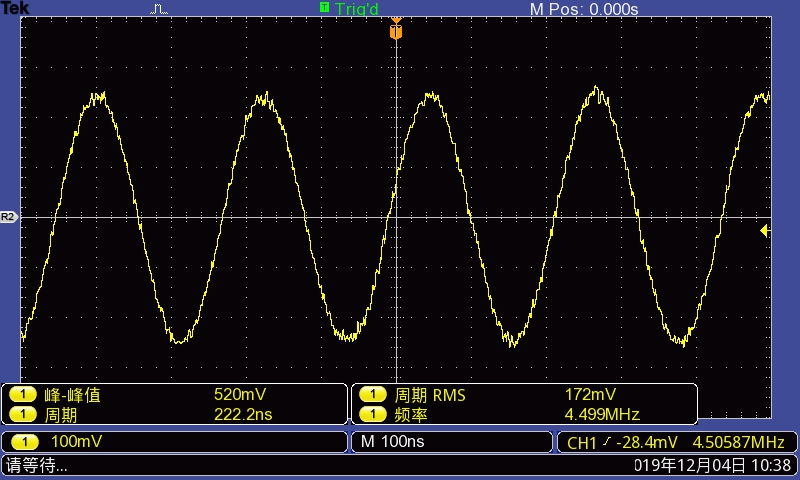
\includegraphics[width=\linewidth]{1.jpg}
		\caption{单调谐小信号放大器}
		\label{fig:单调谐小信号放大器}
	\end{subfigure}
	\quad
	\begin{subfigure}[htbp]{.45\linewidth}
		\centering
		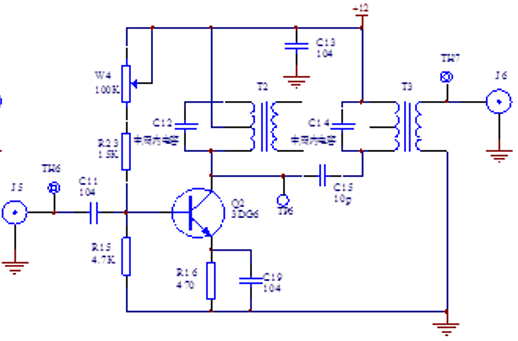
\includegraphics[width=\linewidth]{2.jpg}
		\caption{双调谐小信号放大器}
		\label{fig:双调谐小信号放大器}
	\end{subfigure}
	\caption{高频小信号调谐放大器}
	\label{fig:高频小信号调谐放大器}
\end{figure}

\subsection{单调谐小信号放大器}%
\label{sub:单调谐小信号放大器}

小信号谐振放大器是通信机接收端的前端电路,主要用于高频小信号或微弱信号的线性放大
。其实验单元电路如图\ref{fig:单调谐小信号放大器}所示。该电路由晶体管$ Q_1 $、选频回路$ T_1 $二部分组成。它不仅对高频小信号进
行放大,而且还有一定的选频作用。本实验中输入信号的频率$ f_S = \SI{12}{\MHz} $ 。
基极偏置电阻$ W_2 $、$ R_1 $、$ R_2 $和射极电阻$ R_3 $决定晶体管的静态工作点。可
变电阻$ W_2 $改变基极偏置电阻将改变晶体管的静态工作点,从而可以改变放大器的增益
。表征高频小信号调谐放大器的主要性能指标有谐振频率$ f_0 $,谐振电压放大倍数$
A_\mathrm{v0} $,放大器的通频带BW及选择性(通常用矩形系数$ K_\mathrm{r0.1} $来表
示)等。

\subsection{双调谐小信号放大器}%
\label{sub:双调谐小信号放大器}

双调谐放大器具有频带较宽、选择性较好的优点。双调谐回路谐振放大器是将单调谐回路放
大器的单调谐回路改用双调谐回路。其原理基本相同。

\section{实验步骤}%
\label{sec:\arabic{chapter}实验步骤}

\subsection{单调谐小信号放大器单元电路实验}%
\label{sub:单调谐小信号放大器单元电路实验}

\begin{figure}[htbp]
	\centering
	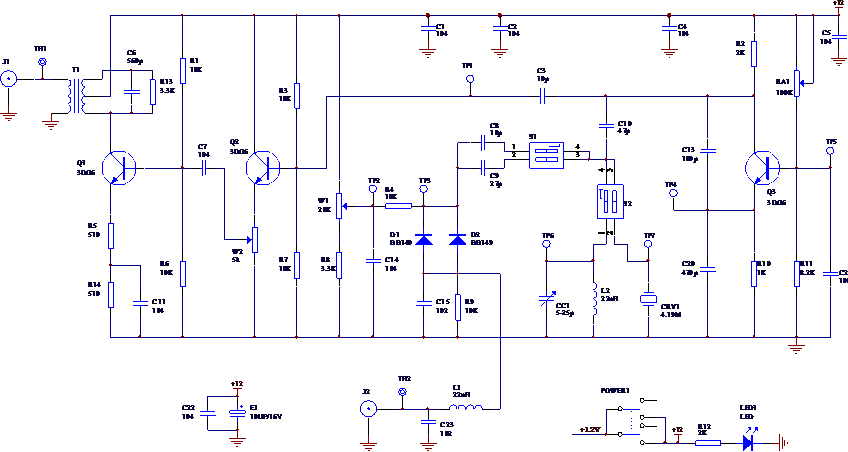
\includegraphics[width=0.6\linewidth]{circuit.png}
	\caption{小信号放大器单元电路实验原理图}
	\label{fig:小信号放大器单元电路实验原理图}
\end{figure}

\begin{enumerate}

	\item 根据电路原理图熟悉实验板电路,并在电路板上找出与原理图相对应的的各
		测试点及可调器件(具体指出)。

	\item 按图\ref{fig:小信号放大器单元电路实验原理图}所示搭建好测试电路。
		\footnote{图中符号\includegraphics[height =
		\ccwd]{\arabic{chapter}/line.png}表示高频连接线}

	\item 打开小信号调谐放大器的电源开关,并观察工作指示灯是否点亮,红灯为
		\SI{+12}{\V}电源指示灯,绿灯为\SI{-12}{\V}电源指示灯。(以后实验
		步骤中不再强调打开实验模块电源开关步骤)

	\item 调整晶体管的静态工作点:在不加输入信号时用万用表(直流电压测量档)
		测量电阻$ R_2 $两端的电压(即$ V_\mathrm{BQ} $)和$ R_3 $两端的
		电压(即$ V_\mathrm{EQ} $),调整可调电阻$ W_2 $,使$
		V_\mathrm{eQ} = \SI{4.8}{\V} $,记下此时的$ V_\mathrm{BQ} $、 $
		V_\mathrm{EQ} $,并计算出此时的$ I_\mathrm{EQ} = V_\mathrm{EQ}
		R_3 $($ R3 = \SI{470}{\ohm} $)。

	\item 按下信号源和频率计的电源开关,此时开关下方的工作指示灯点亮。

	\item 调节信号源\enquote{RF幅度}和\enquote{频率调节}旋钮,使输出端口
		\enquote{RF1}和\enquote{RF2}输出频率为\SI{12}{\MHz}的高频信号。
		将信号输入到3号板的$ J_1 $口,$ \mathrm{TH}_1 $处观察信号峰-峰值
		约为 \SI{100}{\mV}以上,输出在$ J_2 $口,$ \mathrm{TH}_2 $处测试
		观察。

	\item 调谐放大器的谐振回路使其谐振在输入信号的频率点上:将示波器探头连接
		在调谐放大器的输出端即$ \mathrm{TH}_2 $上,调节示波器直到能观察
		到输出信号的波形,再调节中周磁芯与可调电容相互调节使示波器上的信
		号幅度最大,此时放大器即被调谐到输入信号的频率点上。

	\item 测量电压增益$ A_\mathrm{v0} $在调谐放大器对输入信号已经谐振的情况
		下,用示波器探头在$ \mathrm{TH}_1 $和$ \mathrm{TH}_2 $分别观测输
		入和输出信号的幅度大小,则$ A_\mathrm{v0} $即为输出信号与输入信
		号幅度之比。

	\item 测量放大器通频带对放大器通频带的测量有两种方式:

		\begin{enumerate}

			\item 用频率特性测试仪(即扫频仪)直接测量;

			\item 用点频法来测量:即用高频信号源作扫频源,然后用示波
				器来测量各个频率信号的输出幅度,最终描绘出通频带
				特性,具体方法如下:通过调节放大器输入信号的频率
				,使信号频率在谐振频率附近变化(以\SI{20}{\kHz}
				为步进间隔来变化),并用示波器观测各频率点的输出
				信号的幅度,然后就可以在如下的\enquote{幅度-频
				率}坐标轴上标示出放大器的通频带特性。

		\end{enumerate}

\end{enumerate}

\subsection{双调谐小信号放大器单元电路实验}%
\label{sub:双调谐小信号放大器单元电路实验}

双调谐小信号放大器的测试方法和测试步骤与单调谐放大电路基本相同,
只是在以下两个方面稍作改动:

\begin{enumerate}

	\item 调节信号源\enquote{RF幅度}和\enquote{频率调节}旋钮,使输出端口$
		\mathrm{RF}_1 $ 和$ \mathrm{RF}_2 $输出频率为\SI{465}{\kHz}(峰
		-峰值\SI{200}{\mV})。将信号输入到3号板的$ J_6 $口$
		\mathrm{TH}_9 $ 处测试观察,输出在$ J_7 $口$ \mathrm{TH}_{10} $
		处测试观察。

	\item 调节信号源\enquote{RF幅度}和\enquote{频率调节}旋钮,使输出端口$
		\mathrm{RF}_1 $和$ \mathrm{RF}_2 $输出频率为\SI{465}{\kHz}(峰-
		峰值\SI{200}{\mV})。将信号输入到3号板的$ J_6 $口$ \mathrm{TH}_9
		$处测试观察,输出在$ J_7 $口处$ \mathrm{TH}_9 $测试观察。在谐振
		回路的调试时,对双调谐回路的两个中周要反复调试才能最终使谐振回路
		谐振在输入信号的频点上,具体方法是:

		按图\ref{fig:小信号放大器单元电路实验原理图}连接好测试电路并打开
		信号源及放大器电源之后,首先调试放大电路的第一级中周,让示波器上
		被测信号幅度尽可能大,然后调试第二级中周,也是让示波器上被测信号
		的幅度尽可能大,这之后再重复调第一级和第二级中周,直到输出信号的
		幅度达到最大,这样,放大器就已经谐振到输入信号的频点上了。

\end{enumerate}

同单调谐实验,做双调谐实验,并将两种调谐电路进行比较。(以 \SI{2}{\kHz}为步进间
隔来变化)

\section{实验报告要求}%
\label{sec:\arabic{chapter}实验报告要求}

\begin{Exercise}

	整理实验数据,并画出幅频特性。

\end{Exercise}

\begin{Answer}

	数据如表\ref{tab:单调谐电路测量数据}所示。

	\begin{description}

		\item[测量电压增益$ A_\mathrm{V0} $]

			\begin{description}

				\item[单谐振] 信号频率为 \SI{12}{MHz} 时,输入电压
					$ V_1 = \SI{107}{\mV} $,输出电压$ V_2
					= \SI{2.9}{\V} $,求得电压增益为 $
					A_\mathrm{v0} = \dfrac{2.9\times
					1000}{107} = 27.102804 $。

				\item[双谐振]

			\end{description}

		\item[测量放大器同频带]

			\begin{description}

				\item[单谐振] 幅频特性下降为谐振值(
					\SI{12.0}{\MHz})的输出幅度为$ V =
					\SI{4.24}{\V} $对应的信号频率为 $ f_1 =
					\SI{11.58}{\MHz} $,$ f_2 =
					\SI{12.36}{\MHz} $,通频带为放大器的
					\SI{3}{\dB} 通频带$ \mathrm{BW} = |f_2 -
					f_1| = \SI{0.78}{\MHz} $。

				\item[双谐振]

			\end{description}

	\end{description}

\end{Answer}

\begin{table}[htbp]
	\centering
	\caption{单调谐电路测量数据}
	\label{tab:单调谐电路测量数据}
	\csvautobooktabular{tab/\arabic{chapter}/1.csv}
\end{table}

\begin{figure}[htbp]
	\centering
	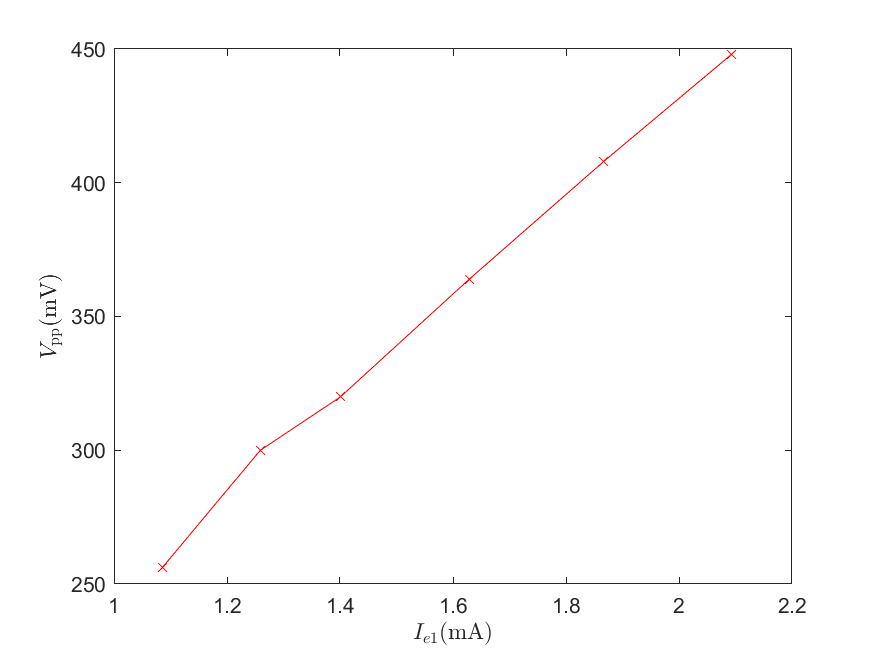
\includegraphics[width = 0.5\linewidth]{1-1.png}
	\caption{单调谐电路测量数据}
	\label{fig:单调谐电路测量数据}
\end{figure}

\section{实验仪器}%
\label{sec:\arabic{chapter}实验仪器}

\begin{table}[htbp]
	\centering
	\caption{实验仪器}
	\label{tab:\arabic{chapter}实验仪器}
	\csvautobooktabular{tab/\arabic{chapter}/BOM.csv}
\end{table}

\end{document}

